\documentclass[12pt,hyperref={pdfpagelabels=false},notes=show]{beamer}

\usetheme[]{FFF}

% Bugfix for pdfpagelables=false
\providecommand\thispdfpagelabel[1]{}

% Standard packages

\usepackage[english,ngerman]{babel}
\usepackage[utf8]{inputenc}
\usepackage{times}

% Setup TikZ

\usepackage{tikz}
\usetikzlibrary{arrows}
\tikzstyle{block}=[draw opacity=0.7,line width=1.4cm]

% Text \us
\usepackage{textcomp}
\usepackage{mathcomp}

% Textpos
\usepackage[absolute,overlay]{textpos}
\setlength{\TPHorizModule}{\paperwidth}
\setlength{\TPVertModule}{\paperheight}

% Blitz-Symbol
\usepackage{stmaryrd}

% Tabellen
\usepackage{multirow}
\usepackage{array}
\usepackage{colortbl}
\definecolor{lightblue}{rgb}{ 0.55, 0.55, 1.00}
\definecolor{lightred}{rgb}{  1.00, 0.35, 0.35}
\definecolor{lightgreen}{rgb}{0.50, 1.00, 0.50}
\newcommand{\ccg}{\cellcolor{lightgreen}}
\newcommand{\ccr}{\cellcolor{lightred}}
\newcommand{\ccb}{\cellcolor{lightblue}}

% Listings
\usepackage{listings}

\setlength{\parindent}{0cm}

%%%%%%%%%%%%%%%%%%%%%% /LAYOUT %%%%%%%%%%%%%%%%%%%%%%%%%%%%


% Author, Title, etc.

\title{Die Technik hinter Freifunk Franken}

\subtitle[ICMP7 Hackercamp]{ICMP7}

\author[Tim Niemeyer]{Tim Niemeyer {\tiny \textless{}tim@freifunk-franken.de\textgreater{}}}

\date[5.8.2014]{05.08.2014}

\newcommand{\zb}{z.\,B.\@}
\newcommand{\us}{~\textmu{}s}
\newcommand{\uv}{~\textmu{}V}
\newcommand{\ms}{~ms}

\begin{document}

\usebackgroundtemplate{\includegraphics[height=\paperheight,width=\paperwidth]{slides_background_title}}

\beamertemplatenavigationsymbolsempty
\begin{frame}[plain,squeeze]
	\maketitle
\end{frame}\addtocounter{framenumber}{-1}

\usebackgroundtemplate{\includegraphics[height=\paperheight,width=\paperwidth]{slides_background}}

\begin{frame}{Inhalt}
    \hspace{0.1\textwidth}
    \parbox[c][0.8\textheight][s]{0.8\textwidth}{
        \tableofcontents
    }
\end{frame}

%%%%%%%%%%%%%%%%%%%%%% CONTENT %%%%%%%%%%%%%%%%%%%%%%%%%%%%

\section{Einleitung}

\begin{frame}{Einleitung}
Der Vortrag gibt zunächst eine kurze allgemeine Einführung zum Thema
Freifunk. Freifunk ist nicht gleich Freifunk, so zeigt der Vortrag
auch die Besonderheiten aus Franken auf.
\end{frame}

\section{Mesh Router}

\begin{frame}{Mesh Router}
%Danach geht der Vortrag auf den inneren Aufbau der Router Software
%(Firmware) ein. Es wird gezeigt, welche Aufgabe ein Router konkret
%zu erfüllen hat.

\begin{block}{
    \only<1-2>{Jeder Knoten ist wie ein großer Switch}
    \only<3-4>{Das Freifunk-Netz besteht aus}
}

\renewcommand{\arraystretch}{1.5}
\begin{tabular}{|c|c|c|c|c|c|c|} \hline
 \multicolumn{7}{|c|}{Bridge} \\ \hline
 \multirow{2}{*}{Managed} & \multicolumn{4}{c|}{\visible<2->{B.A.T.M.A.N}} & \multicolumn{2}{c|}{\multirow{2}{*}{Client-VLan}} \\ \cline{2-5}
 & \visible<3->{Ad-Hoc} & \visible<4->{VPN} & \multicolumn{2}{c|}{\visible<3->{Node-VLan}} & \multicolumn{2}{c|}{} \\ \hline
 \multicolumn{2}{|c|}{Wifi} & \visible<4->{WAN} & \visible<3->{LAN1} & \visible<3->{LAN2} & LAN3 & LAN4 \\ \hline
\end{tabular}

% TODO: Bridge/Managed/Clients grau machen, bei 3-4

\only<1-2>{
        \begin{itemize}
            \item Clients, die sich vor Ort per WLan verbinden
            \item Clients, die sich per Kabel verbinden
            \item<2> Das Freifunk-Netz
        \end{itemize}
}
\only<3-4>{
    \begin{itemize}
        \item Knoten, die sich über WLan verbinden
        \item Knoten, die sich über Kabel verbinden
        \item<4> Knoten, die über VPN verbunden werden
    \end{itemize}
}

\end{block}

\end{frame}


%\begin{frame}{Wifi - Ad-Hoc}
%    % TODO MAC Adressen ???
%\renewcommand{\arraystretch}{1.5}
%\begin{tabular}{|c|c|c|c|c|c|c|} \hline
% \multicolumn{7}{|c|}{Bridge :01} \\ \hline
% \multirow{2}{*}{Managed :01} & \multicolumn{4}{c|}{B.A.T.M.A.N :rr} & \multicolumn{2}{c|}{\multirow{2}{*}{Client-VLan :02}} \\ \cline{2-5}
% & Ad-Hoc :01 & VPN :rr & \multicolumn{2}{c|}{Node-VLan :02} & \multicolumn{2}{c|}{} \\ \hline
% \multicolumn{2}{|c|}{Wifi :01} & WAN :02 & LAN1 :02 & LAN2 :02 & LAN3 :02 & LAN4 :02 \\ \hline
%\end{tabular}
%
%\end{frame}

\begin{frame}{Anschlüsse}
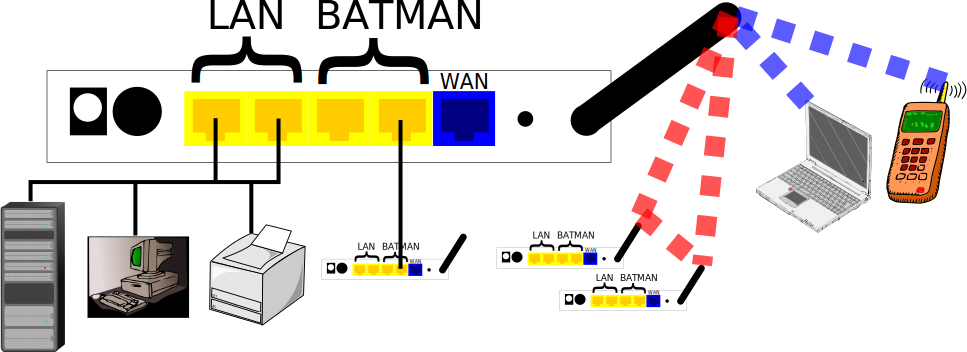
\includegraphics[width=0.75\textwidth]{img/svg/anschluesse.pdf}

An die Client Ports können beliebige Geräte an das Netz angeschlossen werden. Es ist auch mit einem Infrastructure Funknetz verbunden. Die Batman Ports, sowie das AdHoc Netz dienen zur Kommunikation zwischen den Routern. Der LAN-Port kann an ein bestehendes LAN angeschlossen werden und baut darüber einen Tunnel auf.
\end{frame}

\section{Firmware}

%Nachdem der Aufbau der Firmware geklärt ist, soll ein kurzer Abriss
%über den Bauprozess der aktuellen Firmware gezeigt werden. Auch die
%letzten Entwicklungen der Franken eigenen Firmware werden gezeigt
%und erklärt. An dieser Stelle könnten Vorkenntnisse über OpenWrt
%Vorteilhaft sein, sind aber keine Voraussetzung für den Vortrag.

\begin{frame}[fragile]{Firmware}
    \only<1-3>{
        \begin{block}{Wie wird die Firmware gebaut?}
            \begin{itemize}
                \item<1-> git clone \sout{git://git.freifunk-ol.de/ffol/user/reddog/firmware.git}
                \item<1-> cd firmware
                \item<1-> ./buildscript
                \item<3-> ./buildscript selectbsp bsp/board\_wr1043nd.bsp
                \item<3-> ./buildscript selectcommunity community/franken.cfg
                \item<3-> ./buildscript
            \end{itemize}
        \end{block}
    }

    \only<2>{
        \texttt{\scriptsize
            Please select a Board-Support-Package using:\\
            ./buildscript selectbsp
        }
    }

    \only<4>{
        \texttt{\scriptsize
            Working with bsp/board\_wr1043nd.bsp and community/franken.cfg\\[2ex]
            This is the Build Environment Script of the Freifunk Community\\
            Oldenburg.\\
            Usage: ./buildscript command\\
            command:\\
            \hspace{1cm}selectcommunity [communityfile]\\
            \hspace{1cm}selectbsp [bsp file]\\
            \hspace{1cm}prepare\\
            \hspace{1cm}config\\
            \hspace{1cm}build\\
            \hspace{1cm}flash\\
            \hspace{1cm}download\\[2ex]
            If you need help to one of these options just type\\
            ./buildscript command help\\
        }
    }
\end{frame}

\begin{frame}[fragile]{Community File}
    \begin{block}{community/franken.cfg:}
        \scriptsize
        \begin{lstlisting}[gobble=12]
            BATMAN_CHANNEL=1
            ESSID_AP=franken.freifunk.net
            ESSID_MESH=batman.franken.freifunk.net
            BSSID_MESH=02:CA:FF:EE:BA:BE
            NETMON_IP=fe80::ff:feee:1
            VPN_PROJECT=fff
            NTPD_IP=fe80::ff:feee:1%br-mesh
            UPGRADE_PATH=http://[fe80::ff:feee:1%br-mesh]/dev/firmware/current/
        \end{lstlisting}
    \end{block}
\end{frame}

\begin{frame}[fragile]{Board-Support-Package}
    \begin{block}{bsp/board\_wr740n.bsp:}
        \scriptsize
        \begin{lstlisting}[gobble=12]
            machine=wr740n
            target=$builddir/$machine

            board_prepare() {
            }
            board_prebuild() {
            }
            board_postbuild() {
                cp $target/bin/ar71xx/openwrt-ar71[..]-squashfs-*.bin ./bin/
            }
            board_flash() {
                echo "nothing implemented"
            }
            board_clean() {
                /bin/rm -rf $target bin/*$machine*
            }
        \end{lstlisting}
    \end{block}
\end{frame}

\begin{frame}{Board-Support-Package}
    \begin{block}{bsp/wr740n/}
        \begin{itemize}
            \item .config
            \item root\_file\_system/etc/
            \begin{itemize}
                \item rc.local.board
                \item config/
                \begin{itemize}
                    \item board
                    \item network
                    \item system
                \end{itemize}
                \item crontabs/
                \begin{itemize}
                    \item root
                \end{itemize}
            \end{itemize}
        \end{itemize}
    \end{block}
\end{frame}

\begin{frame}{Was macht das Buildscript?}
    \begin{itemize}
        \item Das BSP file wird als dot Script eingeladen
        \item Generiert dynamisches sed-Script
        \begin{itemize}
            \item[$\rightarrow$] Templates mit richtigen Werten zu füllen
        \end{itemize}
    \end{itemize}
\end{frame}

\begin{frame}{Was passiert beim prepare?}
    \begin{itemize}
        \item Sourcen Downloaden
        \begin{itemize}
            \item[$\rightarrow$] separater Source Folder
            \item OpenWRT
            \item Sämtliche Packages
            \begin{itemize}
                \item[$\rightarrow$] ggfs werden Patches angewandt
            \end{itemize}
        \end{itemize}
        \item Ein ggfs altes Target wird gelöscht
        \item OpenWRT wird ins Target exportiert (kopiert)
        \item Eine OpenWRT Feed-Config wird mit dem lokalen Source Verzeichnis als Quelle angelegt
        \item Die Feeds werden geladen
        \item Spezielle Auswahl an Paketen wird geladen
        \item Patches werden angewandt
        \item board\_prepare wird aufgerufen (wird. z.B. für Patches für eine bestimmte HW verwendet)
    \end{itemize}
\end{frame}

\begin{frame}{Was passiert beim build?}
    \begin{itemize}
        \item prebuild
        \begin{itemize}
            \item \$target/files aufräumen
            \item Files aus default-bsp und bsp kopieren
            \item OpenWRT- und Kernel-Config kopieren
            \item board\_prebuild
            \item Templates transformieren
            \item Versionen speichern: \$target/files/etc/firmware\_release
        \end{itemize}
        \item OpenWRT: make
        \item postbuild
        \begin{itemize}
            \item board\_postbuild
        \end{itemize}
    \end{itemize}
\end{frame}

\begin{frame}{Config Targets?}
    \begin{itemize}
        \item prebuild
        \item OpenWRT: make menuconfig ; make kernel\_menuconfig
        \item Speichern, y/n?
        \item Config-Format vereinfachen
        \item Config ins BSP zurück speichern
    \end{itemize}
\end{frame}


\section{VPN}

\begin{frame}{VPN}
Wie die Wireless Mesh Verbindungen zustande kommen geht aus dem
Aufbau der Firmware bereits hervor. Wie jedoch die Knoten
untereinander verbunden werden, soll der Vortrag in einem weiteren
Abschnitt über das verwendete VPN zeigen. Dazu gehört auch die
Aufteilung in Subnetze und die Verbindung der Gateways
untereinander.
\end{frame}

\begin{frame}{Allgemeines}
    \begin{itemize}
        \item Verwendetes VPN: fastd
        \item Wir nutzen keine Verschlüsselung (! :-O)
    \end{itemize}
    \begin{block}{fastd}
        % todo: was ist fastd ?
        There are no server and client roles defined by the
        protocol, this is just defined by the usage.
        \begin{itemize}
            \item Only one instance of the daemon is needed on each
                host to create a full mesh
            \item If no full mesh is established, a routing protocol
                is necessary to enable hosts that are not connected
                directly to reach each other
        \end{itemize}
    \end{block}
\end{frame}

\begin{frame}{Allgemeines}
    \begin{itemize}
        \item fastd Integration durch
        \begin{itemize}
            \item fastdstart.sh auf der Client-Seite
                \footnote{bsp/default/root\_file\_system/etc/fastdstart.sh.tpl}
            \item \$project\_\$hood\_fastd.sh auf der Server-Seite
                \footnote{auf den Gateways (!) Todo: befreien!}
            \item VPN-KeyXchange als Schlüsseltausch
                \footnote{\url{
                    http://git.freifunk-ol.de/projects/ffol/main.git}Todo refresh!}
        \end{itemize}
        \item Aufteilung in ,,hood''s:
        \begin{itemize}
            \item Stellt ein Layer-II Netz dar
            \item Ein Gateway kann mehrere Layer-II Netze bedienen
        \end{itemize}
    \end{itemize}
\end{frame}

\begin{frame}{\alt<1>{fastdstart.sh}{\$project\_\$hood\_fastd.sh}}
    \begin{itemize}
        \item \only<1>{Testet Internet-Connectivität}
        \item Legt fastd Konfiguration
            /etc/fastd/\$project\only<2>{.\$hood}/ \only<1>{im tmpfs} an:
            \footnote{\$project ist bei uns immer ,,fff''.}
            \begin{itemize}
                \item \$project.conf
                \item up.sh
                \item down.sh
                \item peers/
            \end{itemize}
        \item Erzeugt Pub/Priv-Keypaar
        \item Startet fastd
        \item Meldet sich beim VPN-KeyXchange an
        \item Lädt Liste mit Peers
        \item Refresht fastd
        \item \only<2>{Löscht verwaiste Peers}
    \end{itemize}
\end{frame}

\begin{frame}{VPN-KeyXchange}
    \only<1>{
        \begin{block}{HTTP Schnittstelle}
            \texttt{\tiny
                http://mastersword.de/\textasciitilde{}reddog/\$project/?mac=\$mac\&name=\$hostname\&port=\$port\&key=\$pubkey
            }
        \end{block}

        \begin{block}{Rückmeldung}
            \texttt{\tiny
                \#\#\#\#romauplink.conf\\
                \#name "romauplink";\\
                key "9a8ee8b797eed5d3b06778c47fe670987a0eda791ca557da56e6198be45f24c6";\\
                remote ipv4 "109.163.229.254" port 10000 float;\\[2ex]
                \#\#\#\#fff.conf\\
                \#name "fff";\\
                key "543ebc33b36210b10edf62fdb560e3ceac6c64b4ed9ad852f39954522934cd8a";\\
                remote ipv4 "192.168.30.23" port 10000 float;\\[2ex]
                \#\#\#\#90F652F45C34.conf\\
                \#name "ChamHH8Dachboden1";\\
                key "d0e4900fae535d189ef070a527dd00ce2688f3ff7f2b31c4f2846cb658b855fb";\\
                remote ipv4 "93.194.173.193" port 10000 float;\\
            }
        \end{block}
    }
\end{frame}

\section{Gateway}

\begin{frame}{Gateway}
Über die Gateways steht i.d.R. auch eine Internetverbindung zur
Verfügung. Auch die Installation dieser Gateways sollen daher Teil
des Vortrags sein.
\end{frame}

\section{Netmon}

%Ein spezieller Dienst im Freifunk Franken Netz ist das
%Network-Monitoring, kurz Netmon. Netmon selbst soll nicht Teil des
%Vortrags sein, wohl aber die Verbindung zwischen Netmon und den
%Knoten. Dazu zählt zum Beispiel das Handling der Hostnames und das
%Einsammeln der Statusdaten.

\begin{frame}{Netmon}
    % hier mal kurz durch das Netmon durchklicken: Karte, Statistik, Routerliste, Routerstatus

    Knoten
    
    Netmon

    Nodewatcher

    Configurator

\end{frame}

\begin{frame}{Netmon}
    Was muss Netmon kennen, damit es den Router anzeigen kann?

    // Anforderungen an Netmon..

    \begin{itemize}
        \item IP-Adresse des Knotens
            ...
    \end{itemize}
\end{frame}


\begin{frame}{Nodewatcher}
    \begin{itemize}
        \item Erzeugt XML Datei
        \item Läuft alle 5 Minuten
        \item node.data über Webinterface downloadbar
    \end{itemize}
\end{frame}

\begin{frame}{Configurator}
    \begin{itemize}
        \item Knoten kennt Netmon's Link-Local Adresse
        \item Knoten meldet alle 5 Minuten seine MAC Adresse ans Netmon
        \item Netmon meldet dabei zurück, dass der Knoten noch nicht eingetragen wurde
        \item Benutzer ,,übernimmt'' Knoten im Netmon
        \item (Benutzer gibt dem Knoten einen Namen)
        \item Knoten meldet wieder seine MAC an Netmon
        \item Netmon meldet router\_id, update\_hash und api\_key zurück
        \item Knoten trägt nun seine Link-Local Addresse im Netmon ein
        \item Netmon pollt einmal alle 10 Minuten nach router-daten
        \item Knoten pollt alle 5 Minuten nach seinem Hostname
    \end{itemize}
\end{frame}

\section{Aktuelles}

\begin{frame}{Aktuelles}
Zum Abschluss soll ein Überblick über die aktuellen Entwicklungen
gegeben werden. Dazu zählen z.B. die Firmware, ein neues Monitoring,
aber auch Visionen von Richtfunkstrecken und deren performante
Anbindung.
\end{frame}


\section*{}
\begin{frame}{Ende}
    \begin{center}
        Vielen Dank für Eure Aufmerksamkeit	...
     \end{center}
\end{frame}\addtocounter{framenumber}{-1}
	
\section*{}
\include{reserve}

%%%%%%%%%%%%%%%%%%%%%% /CONTENT %%%%%%%%%%%%%%%%%%%%%%%%%%%%

\end{document}
